\documentclass[11pt]{article}
\usepackage[margin=0.88in]{geometry}
\usepackage{amsmath,amssymb,amsthm,mathtools}
\usepackage{microtype}
\usepackage{booktabs}
\usepackage{enumitem}
\usepackage{tikz}
\usepackage[hidelinks]{hyperref}
\setlist{nosep,leftmargin=*}
\newtheorem{theorem}{Theorem}[section]
\newtheorem{corollary}[theorem]{Corollary}
\newtheorem{proposition}[theorem]{Proposition}
\newtheorem{lemma}[theorem]{Lemma}
\theoremstyle{definition}
\newtheorem{definition}[theorem]{Definition}
\newtheorem{warning}[theorem]{Warning}
\theoremstyle{remark}
\newtheorem{remark}[theorem]{Remark}
\newcommand{\Tr}{\operatorname{Tr}}
\newcommand{\Int}{\operatorname{int}}
\newcommand{\dist}{\operatorname{dist}}
\newcommand{\cE}{\mathcal E}
\newcommand{\cT}{\mathcal T}
\newcommand{\cR}{\mathfrak R}
\title{Proposed Manuscript Insertions VI\\
Nested-Separator Contact Closure and the Physical Response Cocycle}
\author{Research draft for the marked-width MLC program}
\date{July 2026}

\begin{document}
\maketitle

\begin{abstract}
For the binary direct-decoration pullback system, we prove that the complete
all-depth physical contact history is a Markov state carried by the current
nested puzzle boundary.  Nonconsecutive shell bypasses are recovered exactly
when the accumulated prefix is glued to the next shell; no all-pairs historical
contact graph and no no-bypass assumption are needed.  After normalization by
the actual univalent branches, the structural contact state is a finite mask
with an explicit recursion.  We construct the exact prefix-to-cell Dirichlet
response recursion, extend it to every already frozen finite protected-collar
inventory, and retain all word-dependent presentation maps in co-moving
coordinates.  The resulting contact-aware response cocycle exposes the next
major obstruction: universal response/Value compactness and a strict mixed
transition.  These results do not prove MBTT, UPTCR, or MLC.
\end{abstract}

\section{Direct-decoration system}
Let $P$ be the direct-decoration puzzle piece, let $g=f^q$, and use only the
binary univalent pullbacks
\[
 Q_L,Q_R\subset P,\qquad g:Q_a\to P,
 \quad a\in\{L,R\}.
\]
Write $\phi_a=(g|_{Q_a})^{-1}$.  For a word
$w=a_1\cdots a_m$, put
\[
 D_w=\phi_{a_1}\circ\cdots\circ\phi_{a_m}(P),
 \qquad h_w=g^m|_{D_w}:D_w\to P.
\]
For one finite address prefix, abbreviate $D_j=D_{a_1\cdots a_j}$ and
$D_0=P$.  Then
\[
 D_0\supset D_1\supset\cdots\supset D_H
 \tag{1.1}
\]
is a nested chain of closed Jordan puzzle disks with finite
ray/equipotential boundary graphs.  No one-arc boundary-intersection hypothesis
is imposed.

\section{Nested-separator Markov property}
Define
\[
 \Omega_j=\Int D_0\setminus D_j,
 \qquad
 S_{j+1}=\Int D_j\setminus D_{j+1}.
 \tag{2.1}
\]
These open sets may be disconnected.

\begin{theorem}[Nested-separator contact theorem]
For every $j<H$:
\begin{enumerate}
\item $\Omega_j\cap S_{j+1}=\varnothing$;
\item
\[
 \overline{\Omega_j}\cap\overline{S_{j+1}}
 \subset\partial D_j;
 \tag{2.2}
\]
\item away from finitely many puzzle vertices, the active interface is
\[
 I_j=(\partial D_j\cap\Int D_0)\setminus D_{j+1};
 \tag{2.3}
\]
\item gluing equal Sobolev traces on $I_j$ reconstructs
$\Omega_{j+1}=\Int D_0\setminus D_{j+1}$ and adds Dirichlet energies;
\item every contact of $\overline{\Omega_j}$ with any future shell lies on
$\partial D_j$.
\end{enumerate}
\end{theorem}

\begin{proof}
The two open sets lie on opposite sides of the closed disk $D_j$.  A common
closure point is therefore both in $D_j$ and in the closure of its complement,
which proves (2.2).  At a nonvertex point of $\partial D_j$, the prefix
approaches exactly when the point is interior to $D_0$, while the next shell
approaches exactly when the point is not in the closed child $D_{j+1}$.  This
is (2.3).  On each piecewise analytic interface arc, the two sets occupy
opposite sides.  The standard $H^1$ patching theorem identifies the Sobolev
space on the union with pairs having equal traces, and energy is additive.
Every later shell is contained in $D_j$, proving the final assertion.
\end{proof}

\begin{figure}[ht]
\centering
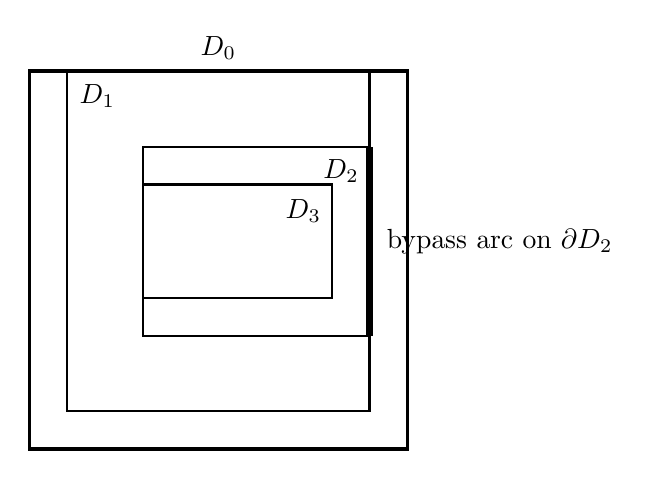
\begin{tikzpicture}[scale=.48]
  \draw[very thick] (0,0) rectangle (10,10);
  \draw[thick] (1,1) rectangle (9,10);
  \draw[thick] (3,3) rectangle (9,8);
  \draw[thick] (3,4) rectangle (8,7);
  \draw[line width=2.4pt] (9,3)--(9,8);
  \node at (5,10.6) {$D_0$};
  \node at (1.8,9.35) {$D_1$};
  \node at (8.25,7.35) {$D_2$};
  \node at (7.25,6.3) {$D_3$};
  \node[anchor=west] at (9.2,5.5) {bypass arc on $\partial D_2$};
\end{tikzpicture}
\caption{The audit's alternating-attachment bypass.  When $D_3$ is added,
$D_0\setminus D_2$ is the accumulated prefix, and the entire bypass is an
ordinary part of the current separator $\partial D_2$.}
\end{figure}

\begin{corollary}[All-depth bypass capture]
Every nonconsecutive shell contact is captured at the unique stage at which it
becomes a prefix--next-shell contact.  Historical shell-pair data are not
needed for exact response composition.
\end{corollary}

\section{Frozen protected collars and obstacles}
Let $Z\subset\overline{D_0}$ be a finite horizon-frozen union of regular
protected collar tails, obstacle walls, ideal-interval walls, and electrode
arcs.  Put
\[
 \Omega_j^Z=(\Int D_0\setminus D_j)\setminus Z,
 \qquad
 S_{j+1}^Z=(\Int D_j\setminus D_{j+1})\setminus Z.
\]

\begin{theorem}[Frozen-collar separator calculus]
Every common contact of $\overline{\Omega_j^Z}$ and
$\overline{S_{j+1}^Z}$ lies on $\partial D_j$.  The genuine glue is the part
of $I_j$ not declared forbidden by $Z$.  Every boundary component of $Z$ is
retained with its declared side-port or boundary-condition type.
\end{theorem}

\begin{proof}
Deleting $Z$ can remove approach regions but cannot create a point approached
from both sides of the closed separator away from $\partial D_j$.  Subdivide
$I_j$ at the finite set of intersections with $Z$ and apply the regular
interface patching theorem on the remaining arcs.
\end{proof}

\section{Persistence and finite contact mask}
Take the finite common refinement of $\bigcup_{j=0}^H\partial D_j$, and call
a connected open arc after vertex deletion a boundary atom.

\begin{theorem}[Persistence intervals]
For a boundary atom $J$, the set
\[
 \{j:J\subset\partial D_j\}
\]
is empty or an integer interval.
\end{theorem}

\begin{proof}
If $J\subset\partial D_i\cap\partial D_k$ with $i<j<k$, then
$D_k\subset D_j\subset D_i$ gives $J\subset D_j$.  A point of $J$ cannot be
interior to $D_j$, since a small disk in $D_j\subset D_i$ would contradict
membership in $\partial D_i$.  Hence $J\subset\partial D_j$.
\end{proof}

\begin{corollary}
A physical boundary port persists through consecutive levels, becomes active
when the nested boundary first leaves it, and never physically reactivates.
\end{corollary}

Now choose a finite root atomization
\[
 \cE=\pi_0(\partial P\setminus V_{\rm geom}),\qquad M=|\cE|,
\]
containing all geometric contact endpoints.  For $a\in\{L,R\}$, let
$A_a\subset\cE$ be the atoms shared by $\partial P$ and $\partial Q_a$, and
refine so that
\[
 \tau_a:A_a\to\cE,\qquad \tau_a(J)=g(J),
 \tag{4.1}
\]
is an atom map.  Define
\[
 R_j=\{J\in\cE:h_{w_j}^{-1}(J)\subset\partial D_0\}.
 \tag{4.2}
\]

\begin{theorem}[Contact-mask recursion]
If $a=a_{j+1}$, then
\[
 \boxed{R_{j+1}=\tau_a(R_j\cap A_a).}
 \tag{4.3}
\]
Consequently the complete structural contact history factors through the
finite automaton
\[
 R\mapsto T_a(R):=\tau_a(R\cap A_a),
 \qquad R\in2^{\cE}.
\]
\end{theorem}

\begin{proof}
A root-shared point of $\partial D_{j+1}$ lies, by persistence, on
$\partial D_j$.  Its $h_{w_j}$-image is simultaneously in $R_j$ and on
$\partial Q_a$, hence in $R_j\cap A_a$; its new label is obtained by applying
$g$.  The converse follows by pulling an atom of $R_j\cap A_a$ back through
$h_{w_j}$.
\end{proof}

\section{Four-way interface classification}
For a state $R$ and symbol $a$, define
\[
\begin{aligned}
 G(R,a)&=(\cE\setminus R)\cap(\cE\setminus A_a),\\
 T(R,a)&=(\cE\setminus R)\cap A_a,\\
 O(R,a)&=R\cap(\cE\setminus A_a),\\
 Z(R,a)&=R\cap A_a.
\end{aligned}
\tag{5.1}
\]

\begin{center}
\begin{tabular}{lll}
\toprule
Class & Physical status & Operation \\
\midrule
$G$ & prefix and cell both approach & glue equal traces and eliminate \\
$T$ & prefix approaches, cell absent & zero-energy transport by $\tau_a$ \\
$O$ & prefix absent, cell approaches & couple to fixed root boundary \\
$Z$ & both absent & retain in new root-shared mask \\
\bottomrule
\end{tabular}
\end{center}

A finite protected overlay further subdivides these atoms but does not create a
fifth structural approach type.

\section{Exact response recursion}
For a finite regular active boundary union $B$, use the intrinsic quotient
trace space
\[
 \cT_\Omega(B)=H^1(\Omega)/\{u:\Tr_Bu=0\}
 \tag{6.1}
\]
with the minimum-energy quotient norm.  Let $q_j$ be the exact closed response
of $\Omega_j^Z$ on fixed external terminals, the active current separator, and
all proof-live side ports.  Let $c_a$ be the exact response of the fixed root
cell $(\Int P\setminus Q_a)\setminus Z_a$.

\begin{theorem}[Geometric separator response recursion]
There is an exact variational update
\[
 q_{j+1}=\cR_{a_{j+1},R_j}(q_j)
 \tag{6.2}
\]
that glues $G$-traces, transports $T$-traces, couples $O$-traces to root-side
data, removes $Z$ from the active trace, retains every proof-live side port,
and minimizes precisely the internal traces.  Its output is the closed
Dirichlet response of the actual domain $\Omega_{j+1}^Z$.
\end{theorem}

\begin{proof}
Transport the next shell by $h_{w_j}$; it is one fixed root cell.  The
separator theorem identifies the complete interface, and (5.1) gives all
approach patterns.  Sobolev patching imposes equality only on $G$.  On $T$ the
same physical arc remains on the child boundary and carries no cell energy.
On $O$ only the cell approaches the fixed root boundary.  On $Z$ neither
conducting side approaches.  Add energies and minimize the internal traces.
The resulting form is the Dirichlet form of the actual glued domain, so it is
closed without invoking an abstract closed-form pushforward theorem.
\end{proof}

\begin{theorem}[DtN Markov sufficiency]
Two prefixes with the same current mask, external labels, separator coordinate
map, and exact response form are indistinguishable by every common finite
future continuation from the binary root-cell catalog.
\end{theorem}

\begin{proof}
Every future step is the deterministic update (4.3), (6.2).  Induct on the
continuation length.
\end{proof}

\begin{corollary}[Geometric live frontier]
Future cells can meet the past only through the current separator.  Its
structural contact frontier has at most $M$ atoms, independent of address
depth.  An old side port absent from the current separator and absent from the
proof ledger is geometrically unreachable by every future cell.
\end{corollary}

\section{Co-moving response cocycle}
The audit's welding objection applies to a global tail uniformization whose
word-dependent endpoint maps are discarded.  Here no such map is discarded.
The actual conformal map $h_{w_j}:D_j\to P$ defines the inner trace coordinate
at every step, and
\[
 h_{w_j}(S_{j+1})=\Int P\setminus Q_{a_{j+1}}.
\]

\begin{theorem}[Contact-aware physical response cocycle]
The complete finite-horizon response is generated by the skew product
\[
 (R,q)\longmapsto
 \bigl(T_a(R),\cR_{a,R}(q)\bigr),
 \qquad a\in\{L,R\},
 \tag{7.1}
\]
on one fixed root-normalized trace category.  All finite-horizon contact and
welding data are exact.  This theorem does not assert norm precompactness or
strict contraction of the response orbit.
\end{theorem}

\section{Contact-neutral and conducting alternatives}
Let $\mathcal C_{\rm contact}$ have vertex set $\cE$ and edge
$J\xrightarrow{a}\tau_a(J)$ whenever $J\in A_a$.

\begin{theorem}[Contact transient/recurrent dichotomy]
Every zero-cell-energy contact trajectory either leaves $\mathcal C_{\rm contact}$ before
visiting more than $M$ distinct atoms, or enters a recurrent strongly
connected component that must be retained as an exact neutral presentation
mode.
\end{theorem}

For one fixed finite-dimensional proof feature space, let $G_\nu\ge0$ be the
accumulated physical-energy Gramian of a word $\nu$ of length $L$, and let
$N_\nu=\ker G_\nu$.

\begin{theorem}[Blockwise Gramian gap]
For one fixed direct-decoration block and one fixed $L$, there is $\gamma_L>0$
such that
\[
 \langle G_\nu x,x\rangle
 \ge \gamma_L\dist(x,N_\nu)^2
 \tag{8.1}
\]
for every admissible word $\nu$ of length $L$.
\end{theorem}

\begin{proof}
There are finitely many words and finite-dimensional Gramians.  Take the
minimum of all positive eigenvalues of the nonzero Gramians.
\end{proof}

\begin{warning}
The constant $\gamma_L$, the feature dimension, and $M$ are block-dependent.
Uniform control over unbounded decorations is not proved.
\end{warning}

\section{Promotion boundary and next theorem}
The results prove the split node
\[
 \boxed{\texttt{PHYSICAL\_END\_SEPARATOR\_CONTACT\_REALIZATION}}.
\]
They also prove the exact finite-horizon response calculus for every already
frozen finite protected inventory.  They do not construct the universal
future inventory or prove compactness of the response/Value orbit.  Hence the
broad collar gate, H2, MBTT, UPTCR, and MLC remain open.

The next major theorem is
\[
\boxed{
\texttt{CONTACT\_AWARE\_RESPONSE\_COCYCLE\_COMPACTNESS\_AND\_VALUE\_OBSERVABILITY}.
}
\]
It must retain recurrent contact modes, prove a universal observability gap on
the transient complement, factor every WAD and Value observable through a
uniformly controlled quotient, compare primitive/neutral/virtual charts in one
gauge, and dominate the full discounted error by a strict complete-block
margin.  This is the direct bridge from the physical geometry to H2 and MBTT.

\end{document}
